\section{Gestione dei dataset forniti}
Da questa sezione in poi il tirocinio entrò nella sua seconda fase di durata 1 mese e le succesive
sezioni e sottosezioni, inclusa la medesima, saranno in ordine cronologico di lavoro.

L'obbiettivo di questa sezione è spiegare le scelte applicative che sono state attuate
per l'elaborazione dei dataset e descriverne il loro contenuto, per 
riuscirne a capire le analisi, le soluzioni ed i risultati ottenuti nelle seguenti sezioni. 




\subsection{Descrizione dei dataset}
Durante il tirocinio sono stati forniti più dataset.
Ogni dataset era relativo ad un paziente, sano o patologico, con una specifica camminata,
più nel dettaglio i dataset erano relativi a camminate normali, sulle punte o tacco punta.
Ogni dataset era formato da più serie temporali, quindi indicizzate nel tempo, relative
alla posizione di un particolare giunto (esempio: piede destro, piede sinistro, naso \dots)

\paragraph{Campionamento dei dati} I dati relativi ad ogni dataset sono stati ottenuti girando un video del soggetto in posizione
laterale e lasciato camminare, avanti ed indietro per un corridoio, davanti all'obiettivo della telecamera. 
Successivamente, i video registrati, sono stati analizzati utilizzando una libreria open source che, con un algoritmo
di machine learning, riconosce i punti relativi alle giunture interessate. Per ogni frame del video
è stato quindi possibile fornire la posizione dei giunti in pixel, sia sull'asse delle
ascisse che delle ordinate, in riferimento al pixel $(0,0)$ del frame analizzato.

Il campionamento dati e la successiva trasformazione di essi in dataset, contenenti le posizioni
dei giunti di ogni soggetto, è stata svolta dal gruppo di ricerca del dipartimento che successivamente
ci ha fornito i dataset elaborati.


\begin{esempio}[Giuntura del naso]
    Se per esempio prendiamo la giuntura del naso relativa ad uno dei dataset, indifferentemente
    dal fatto che esso sia relativo ad un soggetto sano o patologico, essa presenta nel dataset una serie
    chiamata \texttt{x\_naso} e \texttt{y\_naso} che rappresentano rispettivamente 
    la posizione $x$ ed $y$ ad ogni frame acquisito dal video.
\end{esempio}

\subparagraph*{Frequenza di campionamento}
La fotocamera utilizzata per registrare i video ha una frequenza di campionamento di 
$30\mathsf{Hz}$, quindi ogni misurazione è distante dalla successiva circa $33,3\mathsf{ms}$.
Detto ciò la fotocamera riuscirà a captare periodicità che avvengono al massimo ogni $66,6\mathsf{ms}$
($15\mathsf{Hz}$), logicamente per sapere quando un certo evento inizia e finisce abbiamo
bisogno di almeno $2$ misurazioni, più che sufficienti a captare periodicità che risultino
significative all'analisi del movimento di un soggetto.

\subparagraph*{Descrizione delle serie relative ad un dataset}
I giunti forniti dai dataset sono: naso, torace, spalla destra, gomito destro, polso destro, 
spalla sinistra, gomito sinistro, polso sinistro, cresta iliaca, anca destra, ginocchio destro, 
caviglia destra, anca sinistra, ginocchio sinistro, caviglia sinistra, occhio destro, 
occhio sinistro, zigomo destro, zigomo sinistro, piede sinistro ($3$ posizioni), 
piede destro ($3$ posizioni).\\
Per ognuno di questi giunti è presente una misura della posizione sull'asse delle ascisse, 
una misura della posizione sull'asse delle ordinate ed una misura di likelihood cioè un numero
tra $0$ ed $1$ che esprime quanto siamo sicuri di aver trovato il giunto nella posizione giusta
(questa misurazione è stata ignorata).

\subsection{Rinomina delle colonne dei dataset}
I dataset sono stati forniti sprovvisti di una rappresentazione significativa per ogni colonna
quindi, come prima operazione, sono state ridenominate tutte le colonne.

Senza scendere troppo nei dettagli implementativi di come questa operazione è stata eseguita,
poichè una tecnica per la ridenominazione delle colonne è stato fornita nella sezione precedente,
vediamo come i dataset si presentano prima e dopo l'applicazione di essa.

\begin{figure}[H]
    \centering
    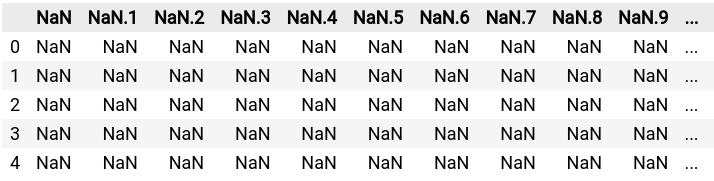
\includegraphics[width=\linewidth,height=2.5cm]{dataset_prima_rinomina.png}
    \caption{Dataset prima della ridenominazione delle colonne.}
    \label{fig:ds_prima_rinomina}
\end{figure}

\begin{figure}[H]
    \centering
    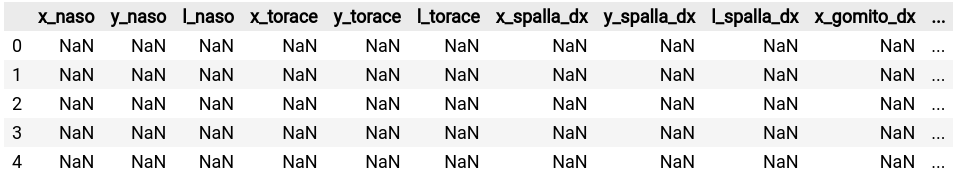
\includegraphics[width=\linewidth,keepaspectratio]{dataset_dopo_rinomina.png}
    \caption{Dataset dopo la ridenominazione delle colonne.}
    \label{fig:ds_dopo_rinomina}
\end{figure}

Come possiamo notare dalle figure~\ref*{fig:ds_prima_rinomina} e~\ref*{fig:ds_dopo_rinomina}
i nomi delle colonne dei dataset sono state ridenominate, esse ora rappresentano meglio
la realtà ed il loro accesso su python facilitato in è possibile accedervi utilizzando
il comando \texttt{dataset\_name.nome\_giunto} invece che \texttt{dataset\_name['nome\_giunto']}.



\subsection{Gestione dei valori nulli}
Nei dataset forniti erano presenti dei valori nulli causati
dall'uscita del soggetto dall'obbiettivo e quindi l'impossibilità, da parte dell'algoritmo
di machine learning, di ottenere una posizione per i giunti interessati.

Essendo che l'obbiettivo finale del tirocinio non è quello di eseguire delle predizioni
sulle serie temporali ma quello di inferire sui dati utilizzando le tecniche
dell'analisi di serie temporali, i valori nulli sono stati semplicemente eliminati.
In questa maniera consideriamo consecutivi dati che effettivamente non lo sarebbero
ma questo non è stato un problema nelle succesive analisi poichè la maggior parte dei 
valori nulli era presente nei momenti in cui il soggetto si girava per eseguire un'ulteriore
camminata davanti all'obiettivo.

Guardiamo ora una esempio di serie prima e dopo l'eliminazione dei valori nulli così da avere
un'idea di come i dati si presentano.

\begin{figure}[H]
    \centering
    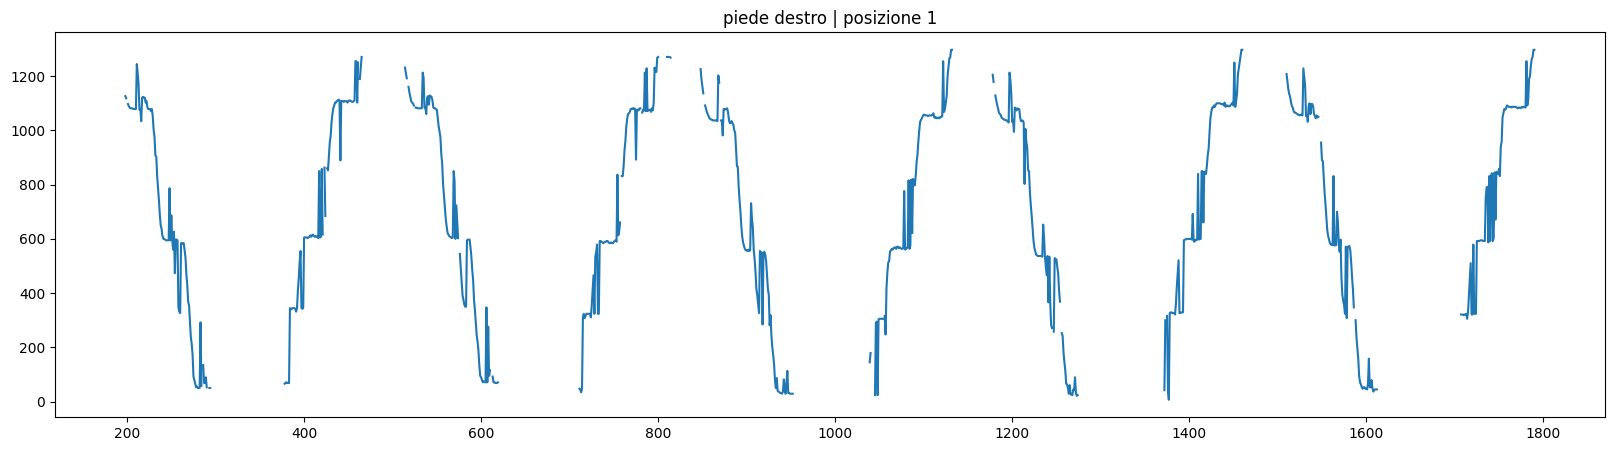
\includegraphics[width=\linewidth,height=4.7cm]{piede_dx_nan.png}
    \caption{Piede destro posizione $1$ con valori nulli.}
    \label{fig:piede_dx_1_nan}
\end{figure}

\begin{figure}[H]
    \centering
    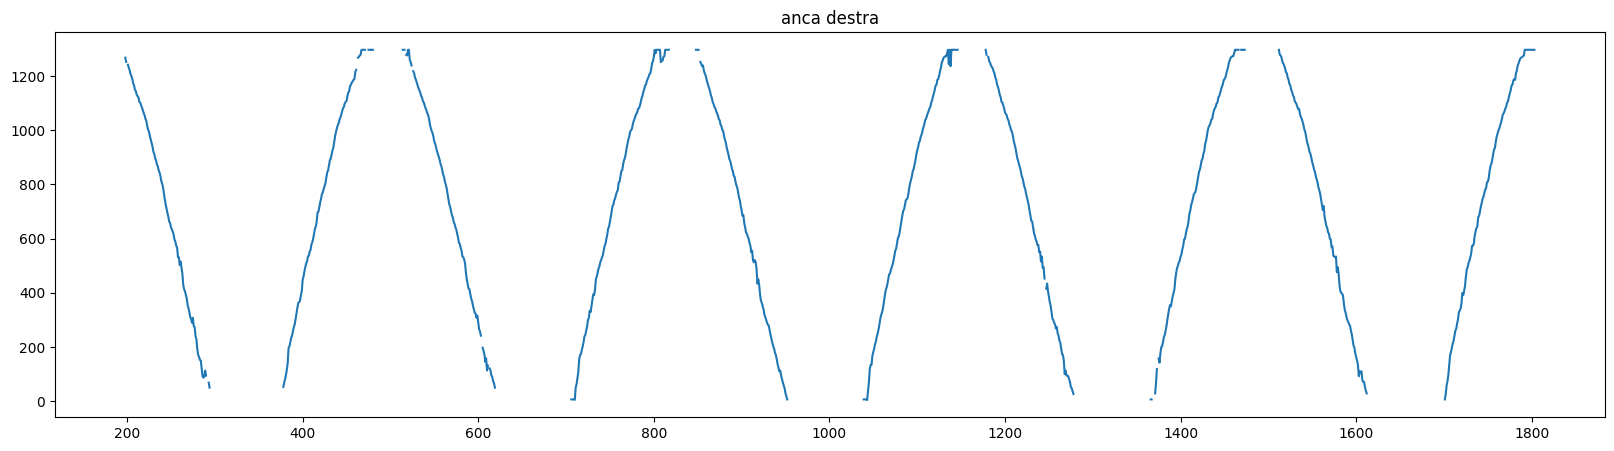
\includegraphics[width=\linewidth,height=4.7cm]{anca_dx_nan.png}
    \caption{Anca destra con valori nulli.}
    \label{fig:anca_dx_nan}
\end{figure}

Come possiamo notare dai grafici in figura~\ref*{fig:piede_dx_1_nan} e~\ref*{fig:anca_dx_nan}
le serie contengono valori nulli nei punti in cui il soggetto esce dall'obiettivo girandosi
per un'altra camminata davanti all'obiettivo.

\begin{figure}[H]
    \centering
    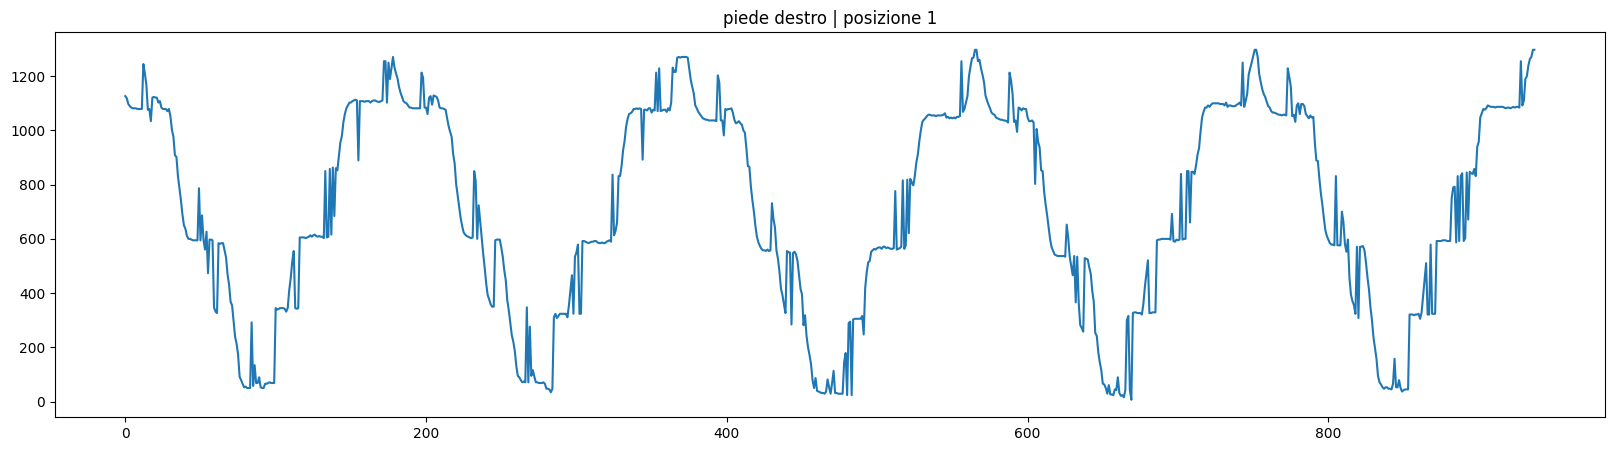
\includegraphics[width=\linewidth,height=4.7cm]{piede_dx_no_nan.png}
    \caption{Piede destro posizione $1$ senza valori nulli.}
    \label{fig:piede_dx_1_no_nan}
\end{figure}

\begin{figure}[H]
    \centering
    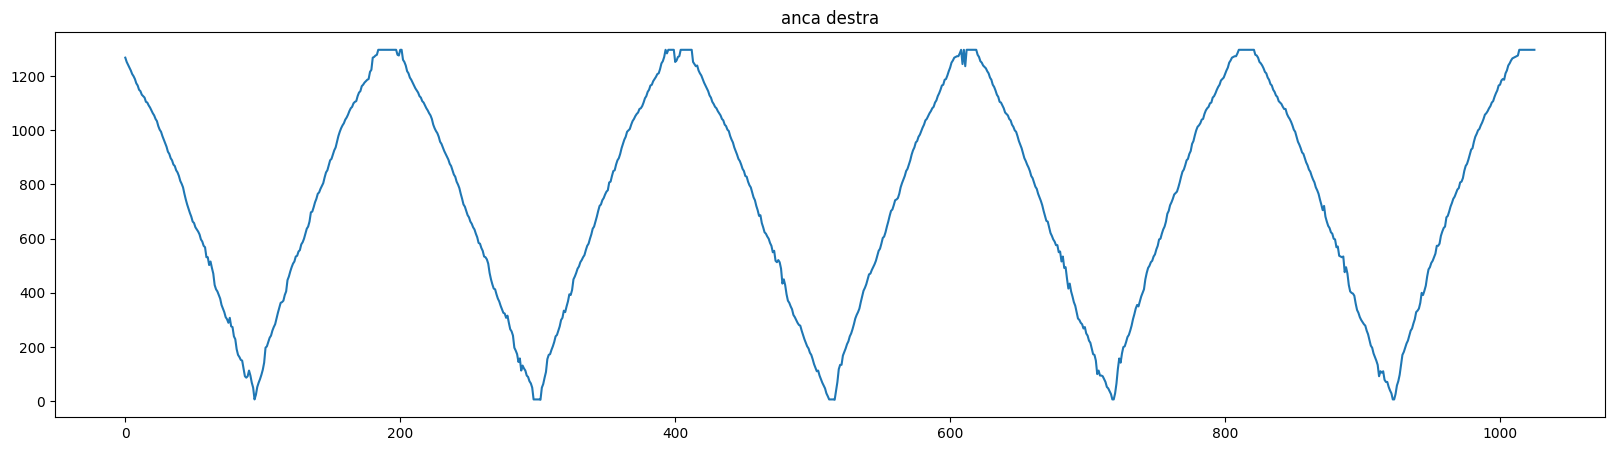
\includegraphics[width=\linewidth,height=4.7cm]{anca_dx_no_nan.png}
    \caption{Anca destra senza valori nulli.}
    \label{fig:anca_dx_no_nan}
\end{figure}

Guardando i grafici rappresentati in figura~\ref*{fig:piede_dx_1_no_nan} e~\ref*{fig:anca_dx_no_nan}
possiamo notare come i valori nulli sono stati eliminati considerando così ogni camminata 
davanti all'obiettivo continua.


\subsection{Scelta dell'indice di tabella per ogni dataset}
Un'osservazione che nasce spontanea dall'osservazione dei grafici in figura
~\ref*{fig:piede_dx_1_nan},~\ref*{fig:anca_dx_nan},~\ref*{fig:piede_dx_1_no_nan}
e~\ref*{fig:anca_dx_no_nan} e dalle tabelle in figura~\ref*{fig:ds_prima_rinomina}
e~\ref*{fig:ds_dopo_rinomina} è che i dataset non sono indicizzati nel tempo utilizzando
la classica indicizzazione come \texttt{anno/mese/giorno ora:minuti:secondi} ma sono indicizzati
in base al frame di acquisizione quindi al numero di riga della tabella.
Questo non è un problema dal punto di vista dell'analisi di ogni serie poichè noto il frame
di acquisizione e la frequenza di campionamento si riuscirà facilmente a risalire ai secodni.

Nel nostro caso, sapendo che i dati sono stati acquisiti con una frequenza di campionamento di 
$30\mathsf{Hz}$, e presa una qualsiasi misurazione ad un certo frame risaliremo al secondo
di tempo con la seguente formula
\[ S_\texttt{frame} = \frac{\texttt{frame}}{30} \]
dove $S_f$ sono i secondi trascorsi dal frame $0$ al frame $\texttt{frame}$ e $\texttt{frame}$ 
è il numero del frame interessato.


\subsection{Filtraggio dei dataset}
Come si può notare dai grafici in figura~\ref*{fig:piede_dx_1_nan},~\ref*{fig:anca_dx_nan},~\ref*{fig:piede_dx_1_no_nan}
e~\ref*{fig:anca_dx_no_nan} le serie dei dataset contengono molto rumore causato da una sbagliata 
lettura della posizione, di ogni giunto, da parte dell'algoritmo di machine learning.

Come spiegato nella precedente sottosezione sul filtraggio il rumore risiede principalemente nelle
alte frequenze di un segnale.

In linea teorica si è pensato che tutte le frequenze più alte di $2\mathsf{Hz}$ possano essere rumore,
quindi in sostanza si andranno ad eliminare tutte le periodicità e movimenti periodici 
che avvengono sotto $0.5 \mathsf{secondi}$. 

Una soluzione migliore sarebbe stata quella di analizzare
ogni serie e, per ciascuna di esse, aplicare un filtro con una frequenza di taglio ottimale così da
non eliminare informazioni importanti. Per lo scopo di questo tirocinio, come verrà spiegato in seguito,
ci soffermeremo sull'analisi dei giunti relativi al piede e quindi una frequenza di taglio di $2\mathsf{Hz}$
potrebbe essere sufficiente a non perdere nessuna informazione importante.


Per fare un esempio pratico supponiamo che l'intervallo di tempo tra due successivi istanti di contatto con il
terreno dello stesso piede (stride), per un soggetto sano, avviene in media ogni $0.8\mathsf{secondi}$,
allora il la frequenza di taglio scelta non elimina la periodicità interessata e riusciremo 
ad individuarla nel grafico.

Nella pratica se applichiamo una frequenza di taglio di $2\mathsf{Hz}$ il segnale rimane con del rumore
e delle periodicità indesiderate, questo è duvuto al cruciale ruolo che svolge l'ordine del filtro.
Dopo svariati tentativi si è riuscito ad ottenere un risultato soddisfacente utilizzando una frequenza
di taglio di $1.2\mathsf{Hz}$ con un ordine di filtro $10$.

Guardiamo ora il risultato finale, ottenuto dopo l'applicazione del filtro con i parametri descritti
precedentemente, ed una serie non filtrata.


\begin{figure}[H]
    \centering
    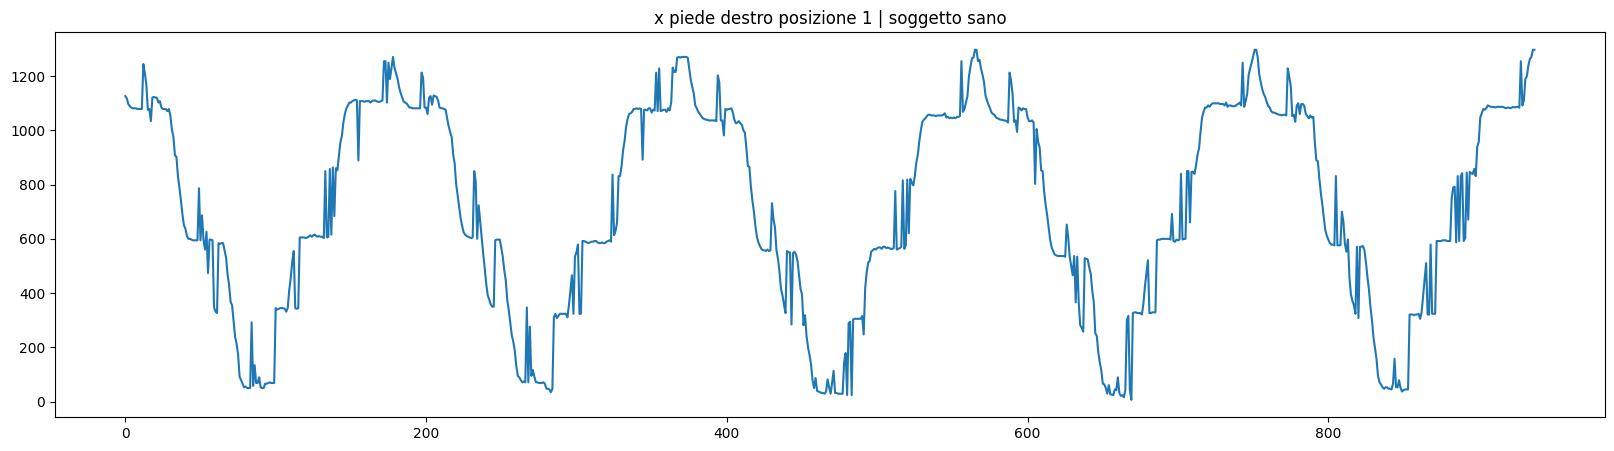
\includegraphics[width=\linewidth,height=4.7cm]{piede_dx_sano_no_filt.png}
    \caption{Piede destro posizione $1$ di un paziente sano prima dell'applicazione del filtro.}
    \label{fig:piede_dx_1_sano_no_filt}
\end{figure}

\begin{figure}[H]
    \centering
    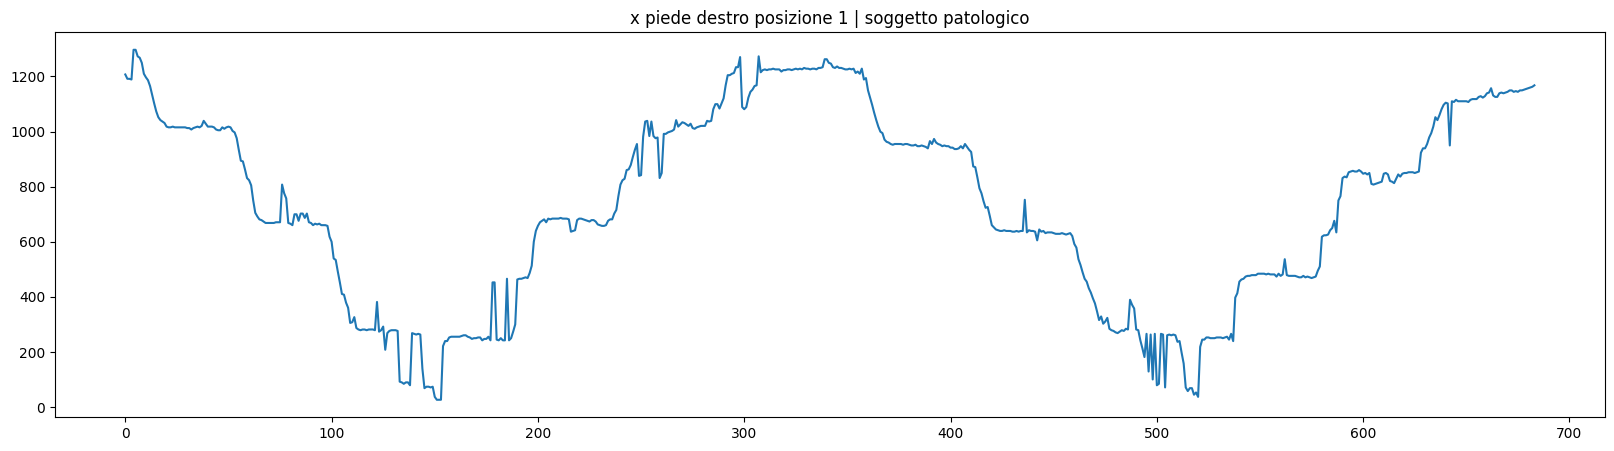
\includegraphics[width=\linewidth,height=4.7cm]{piede_dx_pat_no_filt.png}
    \caption{Piede destro posizione $1$ di un paziente patologico prima dell'applicazione del filtro.}
    \label{fig:piede_dx_1_pat_no_filt}
\end{figure}

Come possiamo notare dai grafici in figura~\ref{fig:piede_dx_1_sano_no_filt} 
e~\ref{fig:piede_dx_1_pat_no_filt} le serie non sono filtrate e contengono molto rumore.

\begin{figure}[H]
    \centering
    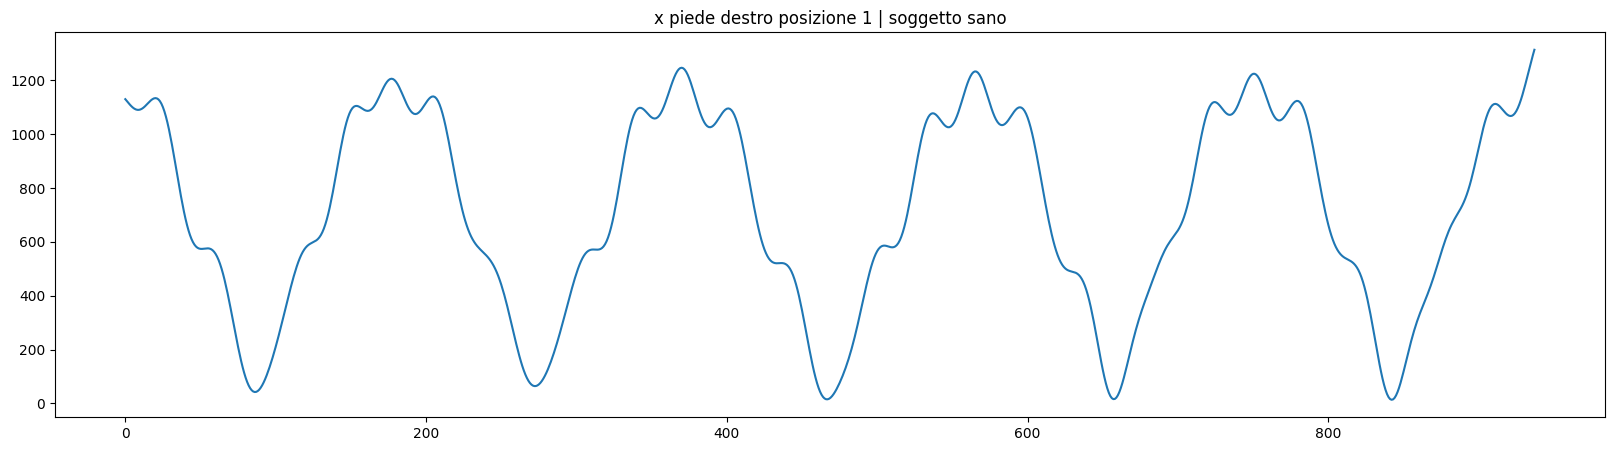
\includegraphics[width=\linewidth,height=4.7cm]{piede_dx_sano_filt.png}
    \caption{Piede destro posizione $1$ di un paziente sano dopo l'applicazione del filtro.}
    \label{fig:piede_dx_1_sano_filt}
\end{figure}

\begin{figure}[H]
    \centering
    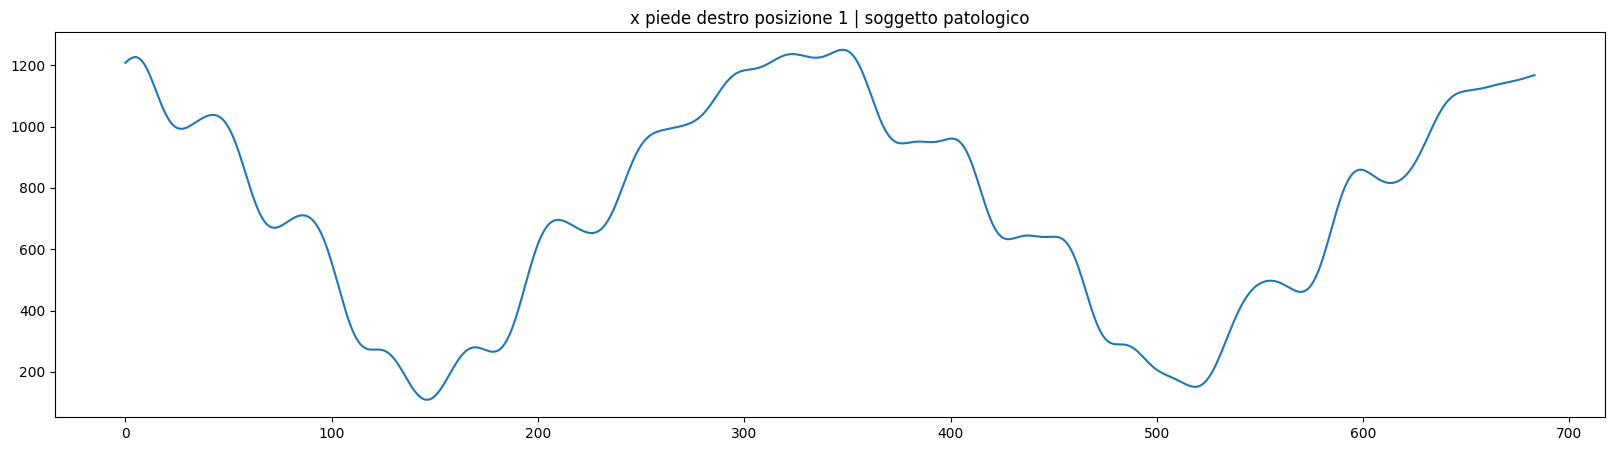
\includegraphics[width=\linewidth,height=4.7cm]{piede_dx_pat_filt.png}
    \caption{Piede destro posizione $1$ di un paziente patologico dopo l'applicazione del filtro.}
    \label{fig:piede_dx_1_pat_filt}
\end{figure}

Dai grafici in figura~\ref{fig:piede_dx_1_sano_filt} 
e~\ref{fig:piede_dx_1_pat_filt} il filtro ha rimosso il rumore e la presenza dello stride
si nota maggiormente.

Un'ulteriore osservazione possibile sui grafici in figura~\ref{fig:piede_dx_1_sano_no_filt},~\ref{fig:piede_dx_1_pat_no_filt},~\ref{fig:piede_dx_1_sano_filt} 
e~\ref{fig:piede_dx_1_pat_filt} è che si nota la presenza della periodicità
relativa ad un'andata e ritorno del soggetto,
essendo che sicuramente avviene più lentamente della periodicità di uno stride, essa
risiede nelle frequenze ``molto basse''. Pensandola da un'ottica dell'analisi
di serie temporali, è presente una stagionalità di periodo $T$ riferita ad una andata
ed a un ritorno del soggetto. Essendo una periodicità non voluta si è deciso di eliminarla
andando a filtrare con un filtro passa alte le frequenze ``bassissime'' o almeno,
abbastanza basse da rimuovere solamente quella periodicità. Dopo qualche tentativo
è stato deciso di utilizzare un filtro passa alte con frequenza di taglio $0.5\mathsf{Hz}$
(periodicità che si ripetono ogni $2\mathsf{secondi}$ e superiori) con un ordine di filtro di $10$.

Vediamo ora i grafici delle due serie rappresentate in figura~\ref{fig:piede_dx_1_sano_filt} 
e~\ref{fig:piede_dx_1_pat_filt} dopo l'ultima fase di filtraggio.

\begin{figure}[H]
    \centering
    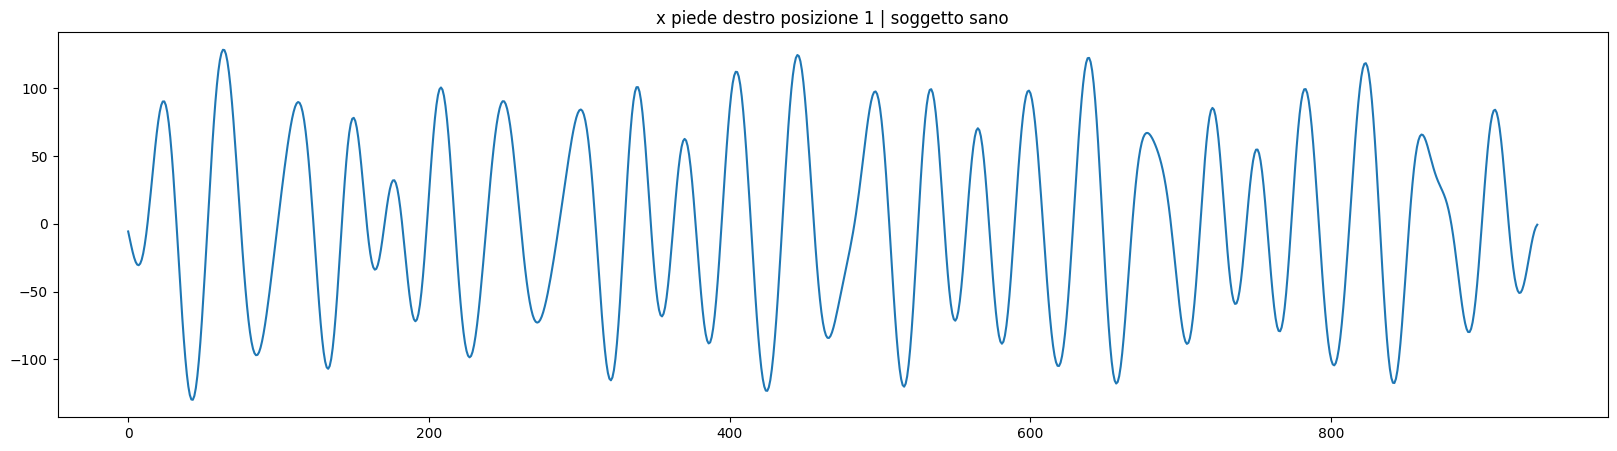
\includegraphics[width=\linewidth,height=4.7cm]{piede_dx_sano_filt2.png}
    \caption{Piede destro posizione $1$ di un paziente sano dopo l'applicazione dell'ultima fase di filtraggio.}
    \label{fig:piede_dx_1_sano_filt2}
\end{figure}

\begin{figure}[H]
    \centering
    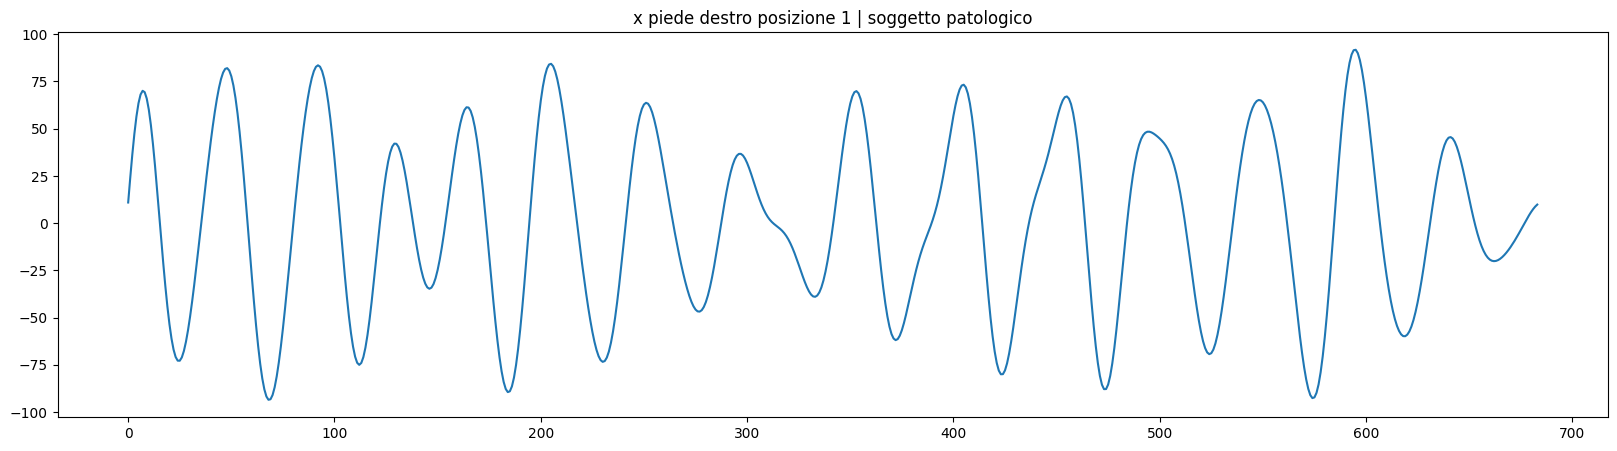
\includegraphics[width=\linewidth,height=4.7cm]{piede_dx_pat_filt2.png}
    \caption{Piede destro posizione $1$ di un paziente patologico dopo l'applicazione dell'ultima fase di filtraggio.}
    \label{fig:piede_dx_1_pat_filt2}
\end{figure}

Come possiamo notare dai grafici in figura~\ref*{fig:piede_dx_1_sano_filt2} e~\ref*{fig:piede_dx_1_pat_filt2}
la componente periodica di andata e ritorno è stata eliminata.